{
% Image scale
\def\imgscale{0.34}

\textsf{Vi vil i det følgende forklare vores tanker bag en meget simpelt
fremgangsmåde, som har til formål at afgøre om et billede opfylder det
gyldne snit.  For at afgøre dette, trækker vi regioner ud af billedet og
vurderer dem efter deres placering, størrelse og form.  Vi siger at et
billede opfylder det gyldne snit, hvis en eller flere interessante
regioner kan siges at ligge i det gyldne snit.  I det følgende vil vi se
på hvornår en region ligger i det gyldne snit samt hvornår vi har med en
interessant region at gøre.
}

\subsection{Regionens placering}
Når vi har trukket regioner ud af et billede og vil afgøre om de ligger
i det gyldne snit, er det indlysende at deres placering har afgørende
betydning.  Vi vil nu komme frem til en definition hvorved man kan
afgøre om en region i billedet er placeret i det gyldne snit.

Vi starter med at se på det meget simple tilfælde, hvor en region
åbenlyst ligger placeret i det gyldne snit.  Et sådan eksempel ses i
figur \ref{pos_naiv_1}, hvor regionen vi betragter er farvet sort.  Den
røde linje markerer det gyldne snit.  Dette farveskema vil være
gennemgående i det følgende.  Det ses at regionen nærmest tangerer
linjen.

\begin{figure}[h]
	\begin{center}
		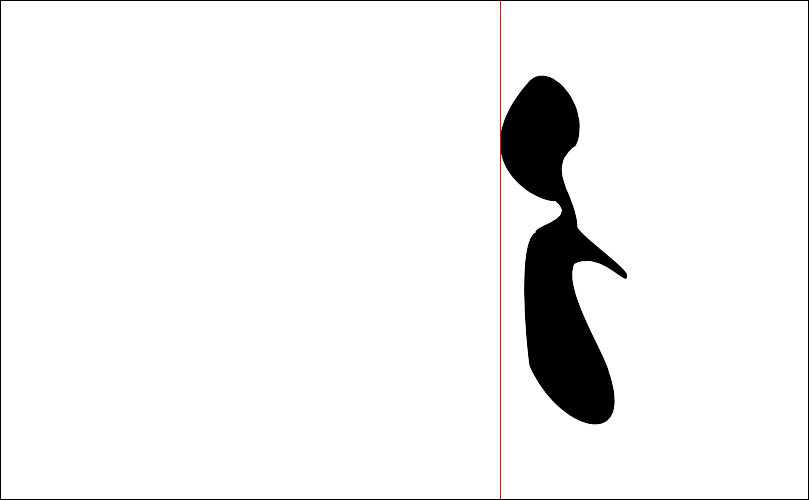
\includegraphics[scale=\imgscale,angle=0]{afsnit/vores_implementation/billeder/naiv_algoritme/naiv_positiv_blob_1}
	\end{center}
	\caption[En positiv region]{En region som tangerer det gyldne snit.
	Denne region er positiv.}
	\label{pos_naiv_1}
\end{figure}

I praksis vil vi dog sjældent have at regioner ligger helt præcist på
snittet.  På grund af den måde, vi trækker regioner ud af billedet på,
kan vi ikke være sikre på at regionen er fyldt helt ud til dens kanter,
fordi der i disse områder stadig er stor overgang i farverne.  Dette
bevirker at en regioner kan blive repræsenteret som mindre end de
virkelig er.  Vi har også, at det gyldne snit baserer sig på det
irrationelle tal $\varphi$ og vi kan derfor ikke regne os helt nøjagtig
frem til vores det egentlige snit ligger.  Vi indfører derfor en margen
hvori vi vil acceptere regioner.  I praksis betyder det at vi ikke
\emph{kun} kigger på den linje der deler billedet ved det gyldne snit,
men faktisk tager vi et bånd, sammensat af en række snit, og bruger
dette bånd som et bredere gyldent snit.  Derved behøver en region ikke
at tangere det gyldne snit helt nøjagtig for at kunne betragtes som en
interessant region. F.eks. vil regionen i figur \ref{pos_naiv_margin_1}
anses som værende placeret i det gyldne snit.  Vær opmærksom på at vores
bånd, rent visuelt i de følgende illustrationer, er stærkt overdrevet.
\begin{figure}[h]
	\begin{center}
		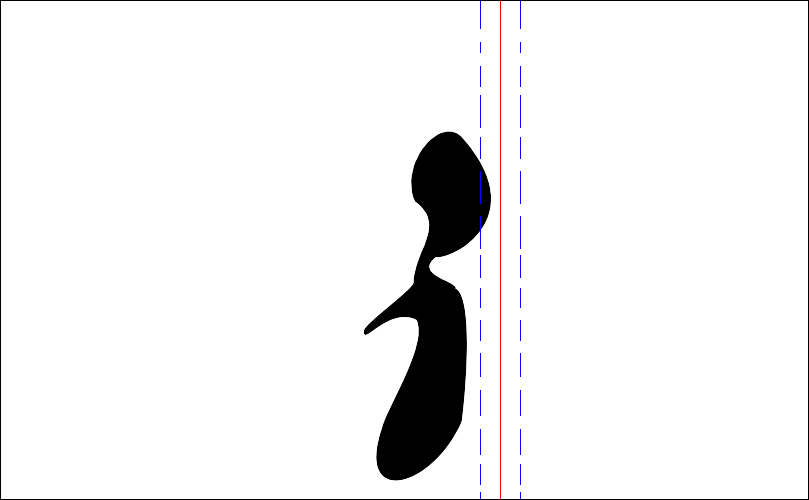
\includegraphics[scale=\imgscale,angle=0]{afsnit/vores_implementation/billeder/naiv_algoritme/naiv_positiv_blob_margin_1}
	\end{center}
	\caption[Positiv region i margen]{En region som
	ligger indenfor en margen af det gyldne snit betragtes som
	positiv. De blå stiplede linjer angiver vores bånd.}
	\label{pos_naiv_margin_1}
\end{figure}

Vi ser nu på det rektangel der der begrænser en region.  En side af
dette rektangel vil vi kalde for en kant.  Vi vil nu komme frem til, at
en region skal have mindst én kant indenfor båndet om det gyldne snit,
før vi kan sige at regionen ligger i det gyldne snit.

\begin{figure}[h]
	\begin{center}
		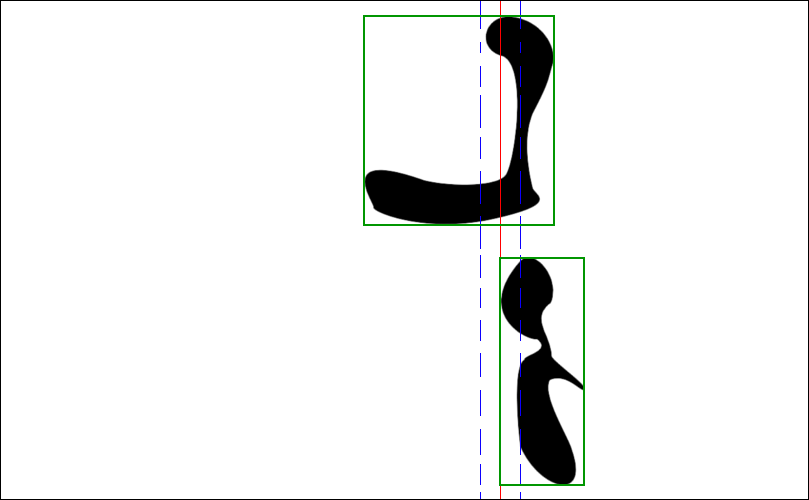
\includegraphics[scale=\imgscale,angle=0]{afsnit/vores_implementation/billeder/naiv_algoritme/bbox_section}
	\end{center}
	\caption[Afgrænsende rektangler]{Den øverste region kan ikke
	siges at ligge i det gyldne snit, da den ikke har nogen kanter
	indenfor båndet. Den nederste region derimod, har én kant
	indenfor båndet og ligger derfor i det gyldne snit.}
	\label{bbox_section}
\end{figure}

\begin{figure}[!h]
	\begin{center}
		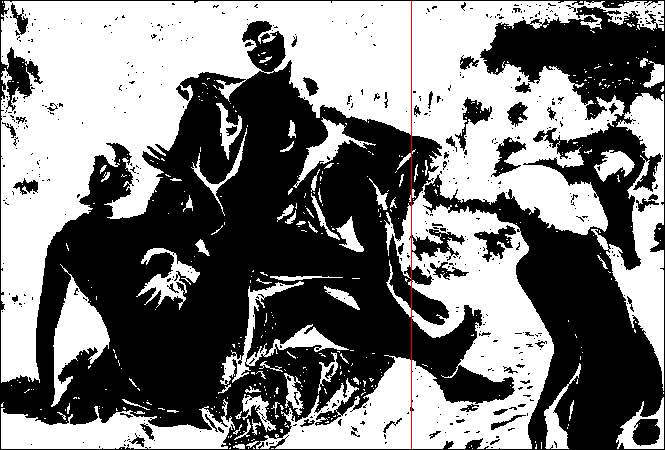
\includegraphics[scale=0.42,angle=0]{afsnit/vores_implementation/billeder/naiv_algoritme/bathers_mockup_blob}
	\end{center}
	\caption[Interessante regioner i praksis]{I praksis vil de
	fundne regioner være langt mere komplekse.}
	\label{realworld_example}
\end{figure}

Med denne definition på hvornår en region kan betragtes som liggende i
det gyldne snit, skal vi blot have en region med en kant indenfor vores
bånd.  I figur \ref{realworld_example} ses hvordan et rigtigt billede
kan tage sig ud når vi vil finde regioner.  Vi ser at der i dette
tilfælde vil blive udvalgt mange små regioner, som egentlig ikke kan
tillægges nogen betydning.  Vi vil nu gå videre og opsætte nogle
kriterier for hvornår en region er interessant.

\subsection{Regionens størrelse}
Når vi skal til at afgøre hvorvidt en region skal tages op til videre
overvejelse er det oplagt at se på størrelsen af regionen.  Vi siger
derfor at en region skal have en vis størrelse før den kan tages i
betragtning.  I praksis vil regionens areal afspejle dens størrelse,
hvor arealet er det antal pixels regionen optager i billedet.  Grænsen
for et acceptabelt areal skal sættes i forhold til billedets størrelse.

Omvendt er vi heller ikke interesseret i at få for store regioner med i
betragtningerne.  F.eks. vil en himmel i et maleri give en ret stor
sammehængende region.  De fleste af sådanne regioner vil dog ikke blive
taget i betragtning fordi de krydser snittet.  Hvis vi kigger på det
meget simple billede i figur \ref{pos_naiv_1} skal man også huske på at
der faktisk vises to regioner. Den sorte skikkelse er en region ligesom
den hvide baggrund er en region.  Baggrunden kan ikke siges at være en
interessant region, hvorfor det er vigtigt at sortere disse regioner
fra.

Indtil videre har vi kun illustreret ét snit i billedet.  Der er
imidlertid tre andre snit hvor vi også kan dele et billede efter det
gyldne snit.  Hvor vi har kigget på et vertikalt snit, vender vi nu
opmærksomheden mod et horisontalt snit.  Det generelle tilfælde vil være
at en region kun er interessant i forhold til enten et vertikalt eller
et horisontalt snit.  Et eksempel på dette ses i figur
\ref{pos_horiz_naiv_margin_1}.  Der kan dog forekomme specialtilfælde,
hvor en region vil være positiv i flere snit, hvilket vi vil komme ind
på i et senere kapitel.
\begin{figure}[H]
	\begin{center}
		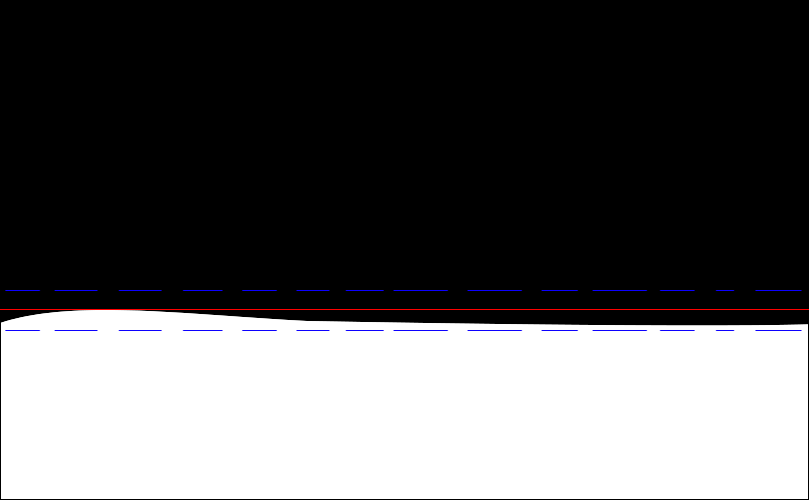
\includegraphics[scale=\imgscale,angle=0]{afsnit/vores_implementation/billeder/naiv_algoritme/naiv_horiz_positiv_blob_1}
	\end{center}
	\caption[Positiv horisontal region]{En positiv region med en
	kant i et horisontalt bånd.}
	\label{pos_horiz_naiv_margin_1}
\end{figure}
Det ses tydeligt at regionen i figur \ref{pos_horiz_naiv_margin_1} ikke
kan tages i betragtning i forhold til et vertikalt snit, da regionen,
uanset snittets placering, vil krydse dette.  Det ses dog at regionen
har en kant indeni et horisontalt bånd og derfor kan klassificeres som
en region der ligger i det gyldne snit.

\subsection{Regionens form}
Regionens form kan give informationer om hvorvidt vi har med en
interessant region at gøre.  I praksis er det dog meget svært at sige
noget om selve den fysiske form af en region, men vi kan sige noget om
dens masse.  En regions masse skal forstås som forholdet mellem
regionens areal og arealet af det rektangel der afgrænser regionen.
Dette forhold giver information om hvor massiv en region er.  En massiv
region vil være mere interessant end en meget spinkel region.  Figur
\ref{region_mass} illustrerer to forskellige regioner med forskellig
masse.
\begin{figure}[h]
	\begin{center}
		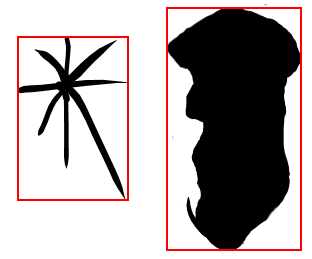
\includegraphics[scale=\imgscale,angle=0]{afsnit/vores_implementation/billeder/naiv_algoritme/bbox_area_ratio}
	\end{center}
	\caption[Regioners masse]{To forskellige regioner med vidt forskellige forhold
	mellem selve regionens areal og arealet af det rektangel der
	afgrænser regionen.}
	\label{region_mass}
\end{figure}
I praksis vil der blive udregnet et tærskel i forhold til et billedes
størrelse for hvor massiv en region skal være for at kunne
karakteriseres som interessant.

\subsection{Sammenfatning af betingelser}
Vi samler nu op på de ovenstående krav for bestemmelse af en interessant
region liggende i det gyldne snit.

\noindent For at en region kan betegnes som interessant og liggende i
det gyldne snit skal den
\begin{enumerate}
	\renewcommand{\labelenumi}{(\alph{enumi})}
	\item have en kant i båndet om det gyldne snit
\end{enumerate}
og regionen må
\begin{enumerate}
	\renewcommand{\labelenumi}{(\alph{enumi})}
	\setcounter{enumi}{1}
	\item \textbf{ikke} krydse båndet der deler billedet ved det gyldne snit;
	\item \textbf{ikke} have et areal mindre end en variabel tærskel der sættes i
		forhold til billedets størrelse
	\item \textbf{ikke} have en masse mindre end variabel tærskel.
\end{enumerate}
Vi har allerede argumenteret for at hvis betingelse $(a)$ er opfyldt
følger det trivielt at betingelse $(b)$ også er opfyldt.  Vi kan da
udlede, at hvis $(a)$ er opfyldt skal vi blot kontrollere $(c)$ og
$(d)$.  Når regionerne i nærheden af det gyldne snit er trukket ud af
billedet er det ligetil at kontrollere betingelserne$(a)$, $(c)$ og
$(d)$ ud fra deres begrænsende rektangel.

Et billede opfylder altså det gyldne snit hvis vi har en eller flere
interessante regioner der ligger i det gyldne snit.  Det er oplagt at
give regioner som er positiv i flere snit større vægt, hvilket vi også
vil komme ind på i et senere kapitel.

\subsection{Begrænsninger}
Denne naive tilgang har nogle begrænsninger.  Den mest åbenlyse er, at
regioner med symmetriakse i det gyldne snit, men med kanter udenfor
båndet ikke vil blive karakterisseret som liggende i det gyldne snit.
Regioner hvor et segment af denne faktisk ligger i båndet, som den
øverste region i figur \ref{bbox_section} hvor den vertikale del faktisk
ligger i snitter, vil ikke blive udvalgt.  Det kræver en videre
segmentering af de fundne regioner før at sådanne regioner vil blive
udvalgt.

}

% vim: set tw=72 spell spelllang=da:
